\chapter{Alpha Wave and Motor Imaginary: the power of masses}

First describe what are alpha waves

Describe the dataset generated

Describe how it was also used to test a public dataset.


\subsubsection{Dataset I - Drowsiness Detection}

%We gather the first dataset  using the EEG EPOC Emotiv Headset and we  access the raw signals using its C++ SDK provided by the manufacturer.  The device sends wirelessly  digitalized 128 Hz sampled EEG information as discrete packets.  Every packet is numbered and the electronic impedance is constantly measured, and delivered as part of the packet information. The wireless transmitter connects to a standard RF dongle which receives the information from  14 channels and forwards it into the PC, particularly to a custom C++ EEG Datalogger program that was developed in-house.  The program is waiting passively until a new packet is received from the dongle, verifying the packet numbering and controlling that the impedance is bellow a certain level, according to the device's documentation \cite{c11}. 

We gather the first dataset using the EEG EPOC Emotiv Headset using the C++ SDK library provided by the manufacturer and an in-house developed program. The device has 14 channels, and a sampling rate of 128 Hz \cite{c11}. Ten random healthy subjects between ages 20-50 were recruited and they accepted to wear the device and to participate in the experiments.  A 30 minutes procedure was required to adjust the headset to each user, in order to decrease the impedance on each electrode. Once the set up was finished, each subject was instructed to sit in a relaxed position. Subsequently, she/he was instructed to watch the screen for 15 seconds, trying to avoid, as much as possible, to abruptly move its body or head.  During that time, a single-trial of 10 seconds-length window of EEG signals data was transferred to a PC and logged into standard binary files. After a 5 minutes pause, the subject was asked to close the eyes avoiding any movement while keeping the same pose for another batch of 15 seconds.  Again, 10 seconds of EEG information were transferred and logged into the PC. This finally gave us a sample of 10 subjects,  2 trial per subject, one for each class, composed of 14 channels, 10-seconds length or 1280 samples per window. Alpha Waves are 8-12 Hz signals, physiologically well consistent across subjects, and they are associated with synchronous inhibitory processes and attention shifting, more prominent while the eyes are closed \cite{c3}. The results of applying a 8-12 Hz band-pass filter and calculating the Power Spectral Density (PSD) across subjects for each channel can be seen in Fig. \ref{figure1}, where the values obtained for class 2 (eyes closed) are higher than the values for class 1 (eyes open), showing that the differentiation information is contained in the frequency-domain.
 
They tend to be more prominent while the eyes are closed and appear stronger in occipital regions. We process this Dataset with a 8-12 Hz band-pass filter, and calculate the Power Spectral Density across subjects for each channel.  In Fig. \ref{psd} it can be seen that the PSD value is greater for the class 2 (eyes closed), showing also that the differentiation information is contained mostly in the frequency-domain.


%As can be seen in Fig. , if we process the Drowsiness dataset with a 8-12Hz band-pass filter and calculate the average power spectral density across subjects and for each channel, we can see how clearly the value corresponding to class 2 (eyes closed) is always higher than the value for class 1 (eyes open), confirming the expected result.  This also verifies how the differentiation information is contained mostly in the frequency-domain.


%   \begin{figure}[thpb]
%      \centering
%      \includegraphics[scale=0.4]{PSDExperiment1VsExperiment2.png}
%      \caption{Power Spectral Density band-passed at 8-12 Hz, for each channel.  The two experiments shows different levels and it can be seen how the experiment 2 for the Drowsiness Dataset has always higher values.  Channels are numbered according to the device numbering system which corresponds to specific electrodes of the 10-20 international system\cite{c6,c11}. }
%      \label{psd}
%   \end{figure}
   
Alpha Waves are 10 Hz signals, physiologically consistent across subjects, and they are associated with synchronous inhibitory processes and attention shifting \cite{c3}. They tend to be more prominent while the eyes are closed and appear stronger in occipital regions ($O_1$ and $O_2$ according to the 10-20 system \cite{c6,c11}). As can be seen in Fig. \ref{psd}, if we process the Drowsiness dataset with a 8-12Hz band-pass filter and calculate the average power spectral density across subjects and for each channel, we can see how clearly the value corresponding to class 2 (eyes closed) is always higher than the value for class 1 (eyes open), confirming the expected result.  This also verifies how the differentiation information is contained mostly in the frequency-domain.



   \begin{figure}[thpb]
      \centering
      \setlength\fboxsep{0pt}
	  \setlength\fboxrule{0.5pt}
      \fbox{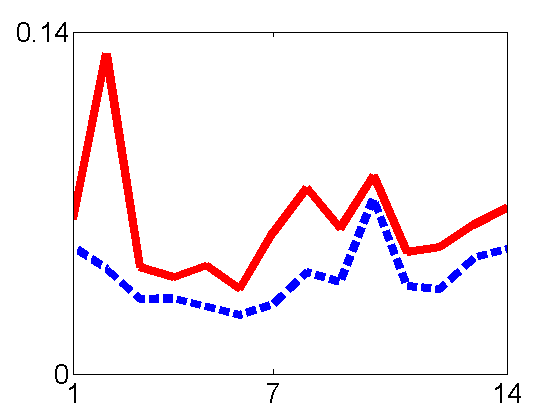
\includegraphics[width=2.5cm, height=1.8cm]{images/PSDExperiment1VsExperiment5.png}}
      \fbox{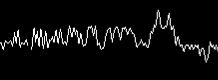
\includegraphics[width=5cm, height=1.8cm]{images/s_1_e_1_c_7_4.png}}
      \caption{PSD values for every channel (x-axis) are being shown for class 1, dashed line, and class 2, solid line, for Dataset I (left). Sample EEG plot image corresponding to the subject 1 (center) for class 1 (eyes open), for the channel 7 ($ O_1 $) }
      \label{figure1}
   \end{figure}
   
   
   


\subsubsection{Dataset II - BCI Competition 2003 IV \textit{self-paced 1s}}
We validated our method against the "BCI Competition 2003, dataset IV \textit{self-paced 1s}" \cite{c51}. This dataset is composed of 28 channels, in 416 epochs of 50 samples per epoch (500 ms length at 100 Hz) each one with the corresponding label, where subjects were asked to type at will a letter on a keyboard with the right or left index finger.  It is based on the Bereitschaftspotential \cite{c52}, which is a Slow Cortical Potential, particularly a slow change in voltages towards a negative potential drift, around 1000-500 ms before the onset of the self-initiated movement.  In this case, the information lies strongly on the time-domain.

This dataset was recorded from a healthy subject during a no-feedback session. She/he sat in a normal chair with relaxed arms resting on the table and fingers in the standard typing position at the computer keyboard. The task was to press with the index and little fingers the corresponding keys in a self-chosen order and timing 'self-paced key typing'. The experiment consisted of 3 sessions of 6 minutes each. All sessions were conducted on the same day with some minutes break in-between. Typing was done at an average speed of 1 key per second.  
